\documentclass {article}
\usepackage{fullpage}
\usepackage{graphicx}
\usepackage{multicol}
\usepackage{hyperref} 


\begin{document}
	
	
	%
	%Title template { Title } {Workplace } {Name/date }
	%\newcommand{\waterlootitle}[3]{
	%\begin{singlespace}
	% \begin{titlepage}
	%
	%  \begin{center}
	
	% \textbf{\MakeUppercase{ University of Waterloo }} \\
	% \textbf{Faculty of Mathematics}
	
	% \vfill  
	
	%{
	% \large
	%\textsc{\textbf{\textit{#1}}}
	% }
	
	%  \vfill
	
	%#2
	
	%\vfill
	
	%prepared by \\[1em]
	%#3
	
	%\end{center}
	
	%\end{titlepage}
	%\end{singlespace}
	%}
	%
	
	%~\vfill
	\begin{center}
		\Large
		
		\textbf{\MakeUppercase{CSC2521 - Computational Design and Fabrication Fall 2017}}
		\vfill  
		
		{
			\Huge
			\textbf{Assignment 1}
		}
		
		{
			\Large
			\textsc{\textbf{Voxelization}}
		}
		
		\vfill
		Name: Lawson Fulton
		
		Student ID: 998262062
		
		Spetember 26, 2017
	\end{center}
	
	\newpage
	\noindent{\Large \bf Results:}
	\begin{description}
		\item[Basic Functionality]:\\
		
		I implemented a basic voxelizer using a single ray cast to determine volume membership. Results for 32x32x32 and 64x64x64 can be seen below for the provided meshes. 
		
		\begin{figure*}[ht!]
			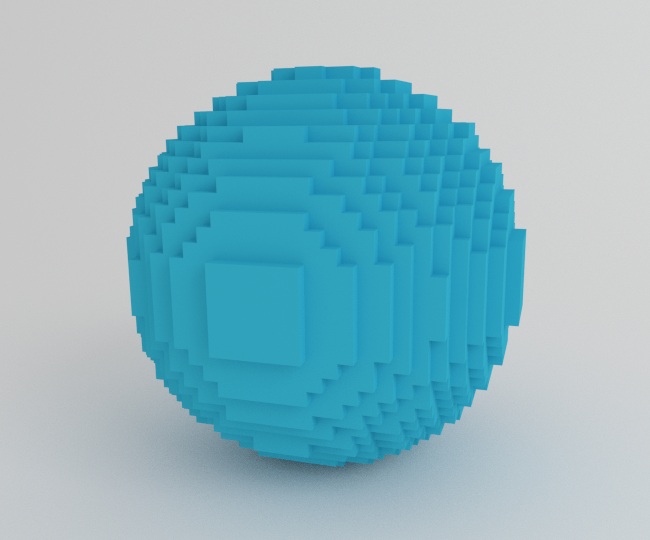
\includegraphics[width=.3\textwidth]{../data/renders/sphere32}\hfill
			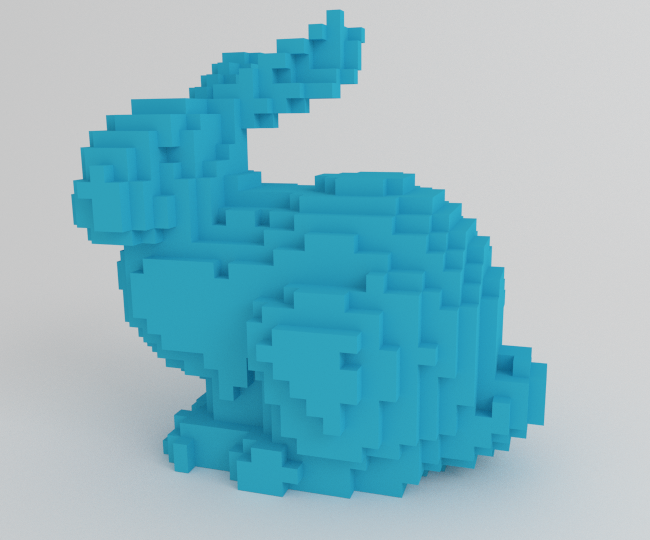
\includegraphics[width=.3\textwidth]{../data/renders/bunny32}\hfill
			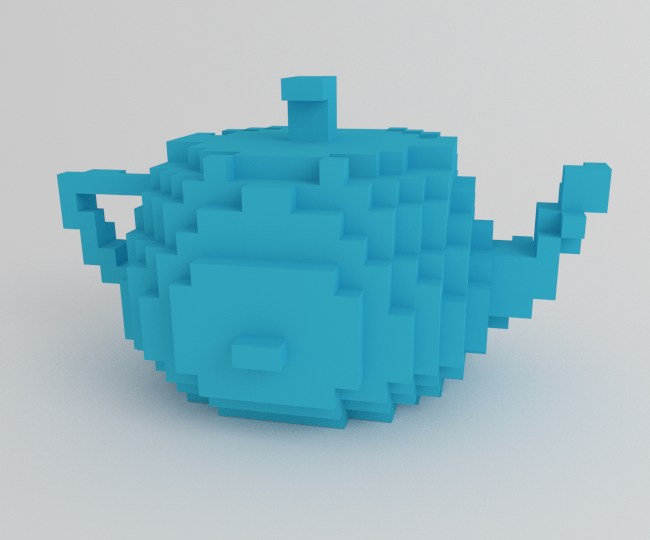
\includegraphics[width=.3\textwidth]{../data/renders/teapot32}
			\caption{34x34x34}
		\end{figure*}
		
		\begin{figure*}[ht!]
			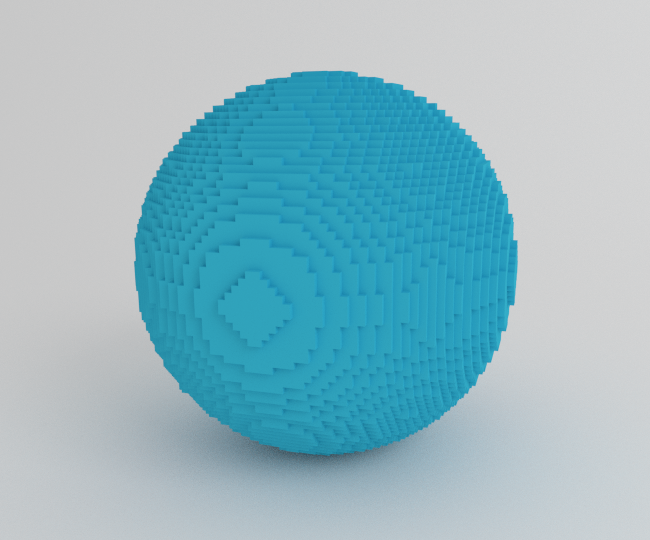
\includegraphics[width=.3\textwidth]{../data/renders/sphere64}\hfill
			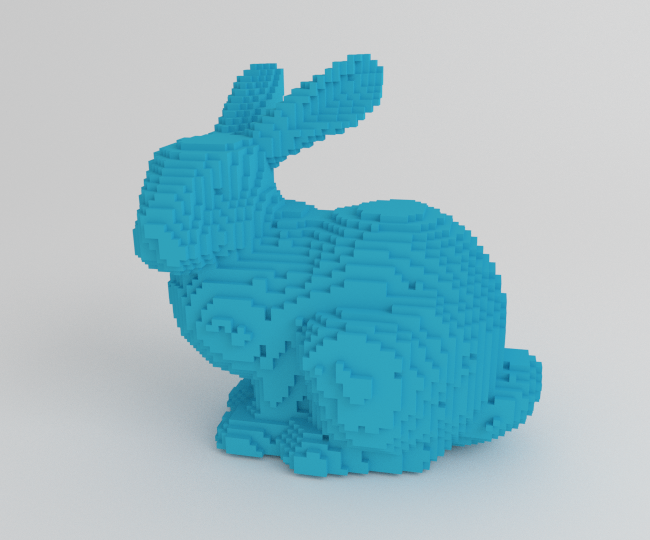
\includegraphics[width=.3\textwidth]{../data/renders/bunny64}\hfill
			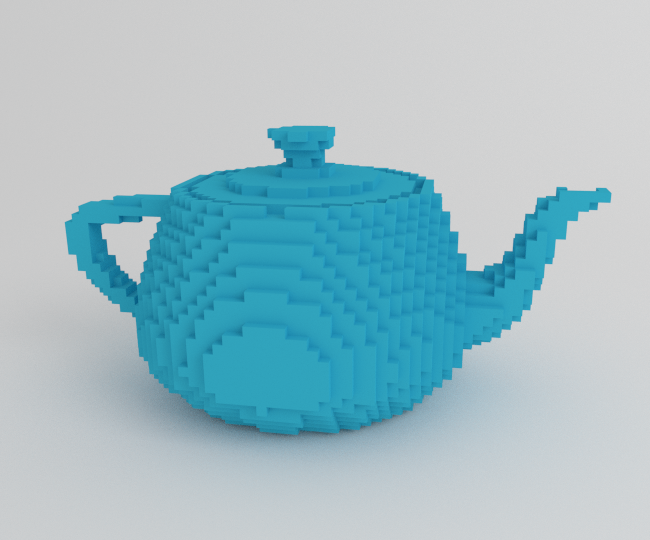
\includegraphics[width=.3\textwidth]{../data/renders/teapot64}
			\caption{64x64x64}
		\end{figure*}


		\item[Extra Functionality]:\\
		
		I also implemented a k-d tree to overcome the main bottleneck of intersecting the ray with every single triangle. This reduces the complexity from $O(mn^3)$ to $O(\log(m)n^3)$ where $m$ is the number of triangles and $n$ the grid resolution.
		
		In figure 3 you can see a model initially containing 100,000 triangles voxelized at a resolution of 128x128x128 that completed in 31s.
		
		Finally, I implemented an averaging of the result of multiple rays cast in different directions. This enables the voxelization of non-closed meshes, as you can see in figure 4.
		
		\begin{figure}
			\begin{center}
				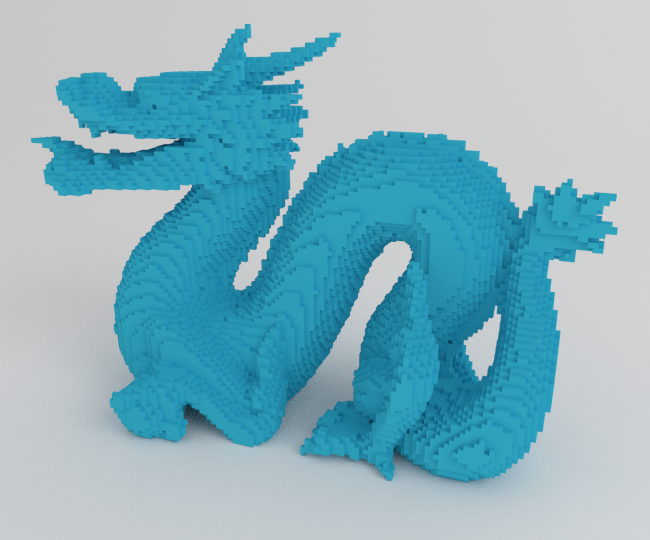
\includegraphics[width=0.6\textwidth]{../data/renders/dragon128}
				\caption{128x128x128 Stanford Dragon}
			\end{center}
		\end{figure}
		
		
		\begin{figure}
			\begin{center}
				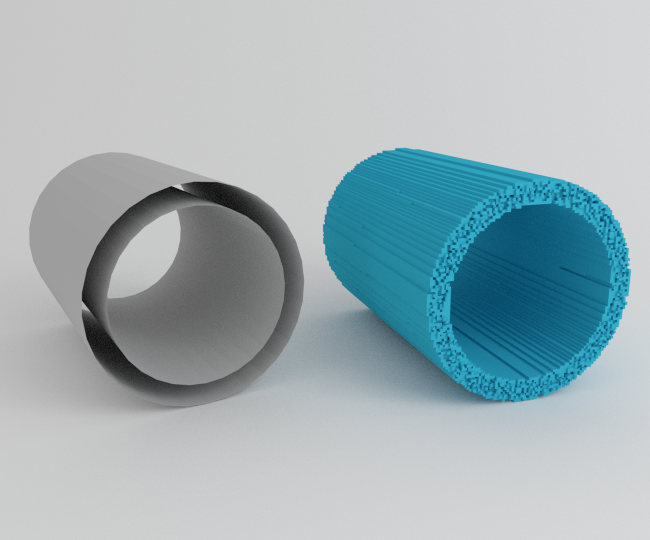
\includegraphics[width=0.6\textwidth]{../data/renders/tubes}
				\caption{Left to right: Source mesh, 128x128x128 voxelization with 30 samples per voxel}
			\end{center}
		\end{figure}
		
		\newpage

		\item[Sources]:\\
		
		1. Fast algorithm for ray-triangle intersection: \href{http://en.wikipedia.org/wiki/M%C3%B6ller%E2%80%93Trumbore_intersection_algorithm}{Moller-Trumbore intersection algorithm}. 
		
		2. Branchless ray to bounding-box intersection algorithm: \href{http://tavianator.com/2011/05/fast-branchless-raybounding-box-intersections/}{http://tavianator.com/2011/05/fast-branchless-raybounding-box-intersections/}.  
		
		3. Stanford 3D scanning repository for Stanford dragon mesh: \href{http://graphics.stanford.edu/data/3Dscanrep/}{http://graphics.stanford.edu/data/3Dscanrep/}. 
		
	\end{description}
	
\end{document}
